\documentclass[aspectratio=169,11pt]{beamer}

% ---------- Packages ----------
\usepackage[T1]{fontenc}
\usepackage{lmodern}
\usepackage{amsmath}
\usepackage{booktabs}
\usepackage{array}
\usepackage{tabularx}
\usepackage{appendixnumberbeamer}
\usepackage[most]{tcolorbox}
\usepackage{tikz}
\usetikzlibrary{positioning,arrows.meta,calc}

% ---------- Colors ----------
\definecolor{SlateTeal}{HTML}{1B4D5C}
\definecolor{WarmAmber}{HTML}{D4A84B}
\definecolor{DeepCharcoal}{HTML}{2C3E50}
\definecolor{SoftCoral}{HTML}{C0534D}
\definecolor{CoolGray}{HTML}{8899A6}
\definecolor{PaleSage}{HTML}{EDF2F0}

% ---------- Safe zone ----------
\newlength{\safezone}
\setlength{\safezone}{1.5cm}

% ---------- Theme ----------
\setbeamersize{text margin left=1.2cm, text margin right=1.2cm}
\setbeamertemplate{navigation symbols}{}
\setbeamercolor{normal text}{fg=DeepCharcoal,bg=white}
\setbeamercolor{frametitle}{fg=SlateTeal}
\setbeamercolor{structure}{fg=SlateTeal}
\setbeamercolor{alerted text}{fg=SoftCoral}
\setbeamercolor{footline}{fg=CoolGray}
\setbeamercolor{button}{bg=PaleSage,fg=SlateTeal}
\setbeamerfont{frametitle}{size=\Large,series=\bfseries}
\setbeamerfont{footline}{size=\scriptsize}
\setbeamertemplate{itemize item}{\color{WarmAmber}\raisebox{0.15ex}{\scriptsize$\blacksquare$}}
\setbeamertemplate{itemize subitem}{\color{CoolGray}\textendash}
\setbeamertemplate{enumerate item}{\color{SlateTeal}\bfseries\insertenumlabel.}

\setbeamertemplate{frametitle}{%
  \vskip18pt%
  \nointerlineskip%
  {\usebeamerfont{frametitle}\usebeamercolor[fg]{frametitle}\insertframetitle\par}%
  \vskip2pt%
  {\color{WarmAmber}\rule{\textwidth}{1.2pt}}%
  \vskip4pt%
}

\setbeamertemplate{footline}{%
  \begin{beamercolorbox}[wd=\paperwidth, ht=18pt, right, rightskip=\safezone]{footline}%
    \usebeamerfont{footline}\insertframenumber\,/\,\inserttotalframenumber\vskip6pt%
  \end{beamercolorbox}%
}

% ---------- Boxes ----------
\newtcolorbox{keybox}[1][]{enhanced, colback=PaleSage, colframe=SlateTeal,
  boxrule=0pt, leftrule=3pt, arc=2pt, left=8pt, right=8pt, top=6pt, bottom=6pt,
  fontupper=\color{DeepCharcoal}, #1}
\newtcolorbox{cardbox}[2][]{enhanced, colback=white, colframe=SlateTeal!35,
  boxrule=0.6pt, arc=2pt, left=6pt, right=6pt, top=4pt, bottom=5pt,
  title={#2}, coltitle=white, colbacktitle=SlateTeal, fonttitle=\bfseries\small,
  fontupper=\footnotesize\raggedright, before upper={\setlength{\itemsep}{1pt}},
  #1}
\newtcolorbox{accentbox}[1][]{enhanced, colback=WarmAmber!12, colframe=WarmAmber,
  boxrule=0.8pt, arc=2pt, left=8pt, right=8pt, top=5pt, bottom=5pt, #1}

\newcommand{\hl}[1]{{\color{WarmAmber}\bfseries #1}}
\newcommand{\muted}[1]{{\color{CoolGray}#1}}
\newcommand{\hy}[1]{\textbf{\textcolor{SlateTeal}{#1}}}

% ---------- TikZ styles ----------
\tikzset{
  stage/.style={draw=SlateTeal, fill=PaleSage, rounded corners=2pt, line width=0.7pt,
    text width=2.55cm, minimum height=1.05cm, align=center, font=\small\bfseries,
    text=SlateTeal, execute at begin node={\hyphenpenalty=10000\exhyphenpenalty=10000}},
  zombie/.style={stage, draw=SoftCoral, fill=SoftCoral!10, text=SoftCoral},
  exitnode/.style={stage, draw=WarmAmber, fill=WarmAmber!18, text=DeepCharcoal},
  note/.style={text width=2.75cm, align=center, font=\scriptsize, text=CoolGray,
    execute at begin node={\hyphenpenalty=10000\exhyphenpenalty=10000}},
  flow/.style={-{Stealth[length=2.2mm]}, line width=0.8pt, color=SlateTeal!70},
}

% ---------- Title info ----------
\title{Who Pays When Firms Keep Losing?}
\subtitle{Workers, Owners, and Debt over the Distress Life Cycle}
\author{Research Proposal}
\date{}

\setbeamertemplate{title page}{%
  \vfill
  \begin{center}
    {\usebeamerfont{title}\Huge\bfseries\color{SlateTeal}\inserttitle\par}
    \vskip8pt
    {\color{WarmAmber}\rule{0.55\textwidth}{1.2pt}}
    \vskip8pt
    {\Large\color{DeepCharcoal}\insertsubtitle\par}
    \vskip22pt
    {\large\color{CoolGray}\insertauthor\par}
    \vskip4pt
    {\small\color{CoolGray}Canadian linked worker--firm--owner data, 2001--2019\par}
  \end{center}
  \vfill
}

\begin{document}

% ======================================================
\begin{frame}[plain]
  \titlepage
\end{frame}

% ======================================================
\begin{frame}{Insurance against losses has to be paid for}
  \begin{columns}[T,onlytextwidth]
    \column{0.52\textwidth}
    \textbf{What we know}
    \begin{itemize}
      \item Workers capture a \hl{small share} of firm gains \muted{(Card et al.\ 2018; Kline et al.\ 2019)}
      \item But they bear a \alert{larger share} of losses, mainly via job loss \muted{(Wang \& Young 2025)}
      \item Firms \hl{partly insure} workers against firm shocks \muted{(Guiso, Pistaferri \& Schivardi 2005; Balke \& Lamadon 2022)}
    \end{itemize}

    \column{0.44\textwidth}
    \begin{keybox}
      \textbf{The gap.}\\[3pt]
      Insurance is not free. When a firm \emph{keeps} losing money, someone funds it:
      \begin{itemize}
        \item owners' equity
        \item new debt
        \item workers, once the firm can no longer pay
      \end{itemize}
      \vspace{2pt}
      \textbf{Who, and when?}
    \end{keybox}
  \end{columns}
\end{frame}

% ======================================================
\begin{frame}{Research question}
  \vspace{4pt}
  \begin{keybox}
    \large When a private firm's value added falls \hl{persistently}, how is the loss divided among
    \textbf{incumbent workers}, \textbf{future workers}, \textbf{owners}, and the firm's \textbf{debt}?
    How does this division change as the firm moves from a first loss into \alert{prolonged distress} and \textbf{exit}?
  \end{keybox}
  \vspace{8pt}
  \begin{enumerate}
    \item \textbf{Timing:} Do losses reach workers immediately, or only after owners' buffers run out?
    \item \textbf{State dependence:} Does a thin financial buffer move losses onto workers sooner?
    \item \textbf{Asymmetry:} Do gains rebuild owners' equity while losses end up with workers?
    \item \textbf{Exit:} When a long-distressed (``zombie'') firm finally dies, who pays?
  \end{enumerate}
\end{frame}

% ======================================================
\begin{frame}{Why it matters, and who cares}
  \begin{columns}[T,onlytextwidth]
    \column{0.315\textwidth}
    \begin{cardbox}{Labor economists}
      \begin{itemize}
        \item \emph{Why} is downside incidence asymmetric?
        \item Where does firm insurance stop?
      \end{itemize}
    \end{cardbox}

    \column{0.315\textwidth}
    \begin{cardbox}{Finance \& zombies}
      \begin{itemize}
        \item Zombie work measures aggregate costs, not workers' incomes
        \item Links debt to worker outcomes
      \end{itemize}
    \end{cardbox}

    \column{0.315\textwidth}
    \begin{cardbox}{Policy}
      \begin{itemize}
        \item Forbearance, bailouts, bankruptcy timing
        \item Survival \hl{moves losses} across time
      \end{itemize}
    \end{cardbox}
  \end{columns}

  \vspace{6pt}
  \begin{accentbox}
    \small\textbf{Benefit of knowing:} does protecting distressed firms protect their \emph{workers}, or only delay and shift the losses?
  \end{accentbox}
\end{frame}

% ======================================================
\begin{frame}{Is the answer obvious? No: theory points three ways}
  \begin{columns}[T,onlytextwidth]
    \column{0.315\textwidth}
    \begin{cardbox}{Owners absorb}
      \textbf{Insurance view}\\[2pt]
      Risk-neutral owners smooth wages; losses hit profits and equity.\\[3pt]
      \muted{Azariadis; Baily; Guiso et al.}
    \end{cardbox}

    \column{0.315\textwidth}
    \begin{cardbox}{Workers bear}
      \textbf{Job-loss view}\\[2pt]
      Firms cut jobs rather than wages; displacement costs are large.\\[3pt]
      \muted{Wang \& Young; Bertheau et al.; Graham et al.}
    \end{cardbox}

    \column{0.315\textwidth}
    \begin{cardbox}{Lenders absorb}
      \textbf{Zombie view}\\[2pt]
      Credit keeps unviable firms alive and \emph{prevents} layoffs.\\[3pt]
      \muted{Caballero, Hoshi \& Kashyap; Acharya et al.}
    \end{cardbox}
  \end{columns}

  \vspace{6pt}
  \begin{keybox}
    \small\textbf{Conjecture:} all three hold, \hl{at different stages}. Owners and debt absorb early losses;
    workers bear them \emph{later}, and \emph{sooner} when buffers are thin. The answer is about \textbf{timing}, which has not been measured directly.
  \end{keybox}
\end{frame}

% ======================================================
\begin{frame}{Approach I: follow losses through the distress life cycle}
  \centering
  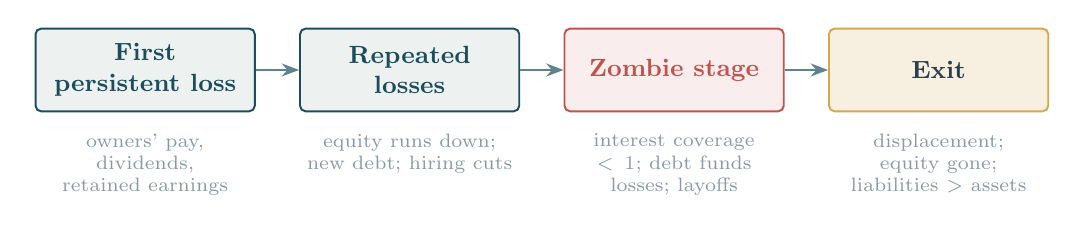
\begin{tikzpicture}[node distance=0.55cm]
    \node[stage]                       (s1) {First persistent loss};
    \node[stage, right=of s1]          (s2) {Repeated losses};
    \node[zombie, right=of s2]         (s3) {Zombie stage};
    \node[exitnode, right=of s3]       (s4) {Exit};
    \draw[flow] (s1) -- (s2);
    \draw[flow] (s2) -- (s3);
    \draw[flow] (s3) -- (s4);
    \node[note, below=0.15cm of s1] {owners' pay, dividends, retained earnings};
    \node[note, below=0.15cm of s2] {equity runs down; new debt; hiring cuts};
    \node[note, below=0.15cm of s3] {interest coverage $<1$; debt funds losses; layoffs};
    \node[note, below=0.15cm of s4] {displacement; equity gone; liabilities $>$ assets};
  \end{tikzpicture}

  \vspace{4pt}
  \begin{columns}[T,onlytextwidth]
    \column{0.48\textwidth}
    \textbf{Data} \muted{(CEEDD, 2001--2019)}
    \begin{itemize}
      \item T4 + ROE: earnings, \hl{layoffs vs quits}, hires
      \item NALMF: value added, \hl{balance sheets}
      \item Schedule 50: \hl{chained ownership} to individuals
    \end{itemize}
    \column{0.48\textwidth}
    \textbf{Design}
    \begin{itemize}
      \item Stacked event studies of persistent value-added falls (and rises)
      \item Matched control firms; intention-to-treat incumbents
      \item Exit: displacement design by distress duration
    \end{itemize}
  \end{columns}
\end{frame}

% ======================================================
\begin{frame}[label=approach2]{Approach II: dollar accounting for every claimant}
  \begin{columns}[T,onlytextwidth]
    \column{0.5\textwidth}
    \textbf{Who gets less income?}\\[-2pt]
    {\small
    \[
      \Delta(\text{VA}+\text{Int}) = \underbrace{\Delta \text{Payroll}}_{\text{workers}}
      + \underbrace{\Delta \text{Int}}_{\text{lenders}}
      + \underbrace{\Delta \Pi + \Delta \text{CCA}}_{\text{owners, gov't}}
    \]}
    \textbf{Who funds the shortfall?}\\[-2pt]
    {\small
    \[
      \Delta \text{Assets} = \underbrace{\Delta \text{Liabilities}}_{\text{debt}} + \underbrace{\Delta \text{Equity}}_{\text{owners}}
    \]}
    \column{0.46\textwidth}
    \begin{keybox}
      \textbf{Estimand:} share of the cumulative loss borne by claimant $g$ by horizon $h$
      \[
        \theta_g(h)=\frac{\sum_{k=0}^{h}\beta^{(g)}_k}{\sum_{k=0}^{h}\beta^{(\text{VA}+\text{Int})}_k}
      \]
      \small Estimated separately for losses and gains, and by the firm's \hl{buffer} at $t-2$.
    \end{keybox}
  \end{columns}

  \vspace{6pt}
  {\small\muted{Value added before interest is the ``pie'': its size does not depend on how it is split.}\par}
  \vspace{2pt}
  \hfill\hyperlink{hyp}{\beamerbutton{Hypotheses}}\hspace{\safezone}
\end{frame}

% ======================================================
\begin{frame}{Contribution}
  \small
  \renewcommand{\arraystretch}{1.25}
  \begin{tabularx}{\textwidth}{>{\raggedright\arraybackslash}p{3.3cm} >{\raggedright\arraybackslash}X >{\raggedright\arraybackslash}X}
    \toprule
    \textbf{Closest paper} & \textbf{What it does} & \textbf{\color{SlateTeal}What this paper adds} \\
    \midrule
    Wang \& Young (2025) & Worker vs owner incidence; asymmetry via job loss (U.S.\ S-corps) & \hl{Financing} of losses; \hl{dynamics} to exit; new hires; layoffs vs quits \\
    Azzalini (2026) & Negative pass-through rises in \emph{recessions} & State = the \emph{firm's own} buffer, on its balance sheet \\
    Malgieri \& Citino (2025) & Constrained firms pass through more & Buffer \emph{evolves} with losses; followed to exit \\
    Graham et al.\ (2023) & Worker losses \emph{at} bankruptcy & The \emph{years before} exit; owners and creditors alongside \\
    Acharya et al.\ (NY Fed) & Zombie credit prevents layoffs (aggregate) & Incomes of zombie firms' \emph{own} workers and owners \\
    \bottomrule
  \end{tabularx}
\end{frame}

% ======================================================
\begin{frame}{Caveats and next steps}
  \begin{columns}[T,onlytextwidth]
    \column{0.48\textwidth}
    \begin{cardbox}{What the design can't do}
      \begin{itemize}
        \item Value-added falls are \alert{not random}: results are incidence \emph{accounting} vs matched firms, not causal effects of exogenous shocks
        \item No lender data: ``debt-funded'' and a creditor-shortfall \emph{bound}, not creditor losses
        \item Zombie status is a \emph{stage}, never a treatment
      \end{itemize}
    \end{cardbox}
    \column{0.48\textwidth}
    \begin{cardbox}{First three months}
      \begin{enumerate}
        \item Check that the accounting identities hold firm by firm
        \item Clean false exits (restructurings, new business numbers)
        \item Does the workers' share \hl{rise with the horizon}? If not, lead with financing + exit
      \end{enumerate}
      \vspace{2pt}
      \muted{Optional: export shocks as an appendix validation.}
    \end{cardbox}
  \end{columns}
\end{frame}

% ======================================================
\appendix
\begin{frame}[plain]
  \vfill
  \begin{center}
    {\Huge\bfseries\color{SlateTeal}Appendix\par}
    \vskip8pt
    {\color{WarmAmber}\rule{0.3\textwidth}{1.2pt}}
  \end{center}
  \vfill
\end{frame}

% ======================================================
\begin{frame}[label=hyp]{Hypotheses}
  \small
  \renewcommand{\arraystretch}{1.25}
  \begin{tabularx}{\textwidth}{p{0.8cm} >{\raggedright\arraybackslash}X >{\raggedright\arraybackslash}p{3.4cm}}
    \toprule
     & \textbf{Prediction} & \textbf{Evidence} \\
    \midrule
    \hy{H1} & Deferred incidence: workers' share of a persistent loss is small at impact and rises over 3--5 years & $\theta_{\text{workers}}(h)$ increasing in $h$ \\
    \hy{H2} & Thin buffers (low equity, prior losses, coverage $<1$) pass losses to workers sooner & Interactions with buffer at $t-2$ (descriptive) \\
    \hy{H3} & Gains rebuild retained earnings; losses end with workers; asymmetry grows with $h$ & $\theta_g(h)$ for rises vs falls \\
    \hy{H4} & Longer distress before exit: more pre-exit erosion, smaller owner loss, bigger creditor gap & Exit design by distress duration \\
    \hy{H5} & Hiring falls before incumbents' earnings & Timing of hires vs incumbents \\
    \bottomrule
  \end{tabularx}
  \vfill
  \hfill \hyperlink{approach2}{\beamerbutton{Back}}\hspace{\safezone}
\end{frame}

% ======================================================
\begin{frame}{Data map: claimant to variables}
  \small
  \renewcommand{\arraystretch}{1.2}
  \begin{tabularx}{\textwidth}{>{\raggedright\arraybackslash}p{3.2cm} >{\raggedright\arraybackslash}X}
    \toprule
    \textbf{Claimant / margin} & \textbf{CEEDD variables} \\
    \midrule
    Incumbent workers & T4 earnings; ROE separation reason (shortage of work vs quit); EI \\
    Future workers & First T4 year at firm; ROE start month (if separated); hires' AKM effects \\
    Owners & Schedule 50 chained shares; owner and family T4 pay; dividends declared; $\Delta$ retained earnings \\
    Debt & Total, current, long-term liabilities; interest and bank charges \\
    Distress stage & Interest coverage; loss carryforward; equity; incorporation date \\
    Exit & Last PD7 remittance month (cleaned of successor firms) \\
    \bottomrule
  \end{tabularx}
\end{frame}

\end{document}
